\section{How to formulate a ration}
\subsection{View Nutrient  List}\label{sec:nutrient_list}
\setcounter{stepcounter}{1}
\paragraph{\arabic{stepcounter}.}On left sidebar menu click \textcolor{ForestGreen}{"Formulate"} then select \textcolor{ForestGreen}{"New Formula"} menu, then you will be redirect to Ration Formulation page.

\begin{figure}[h!]
  	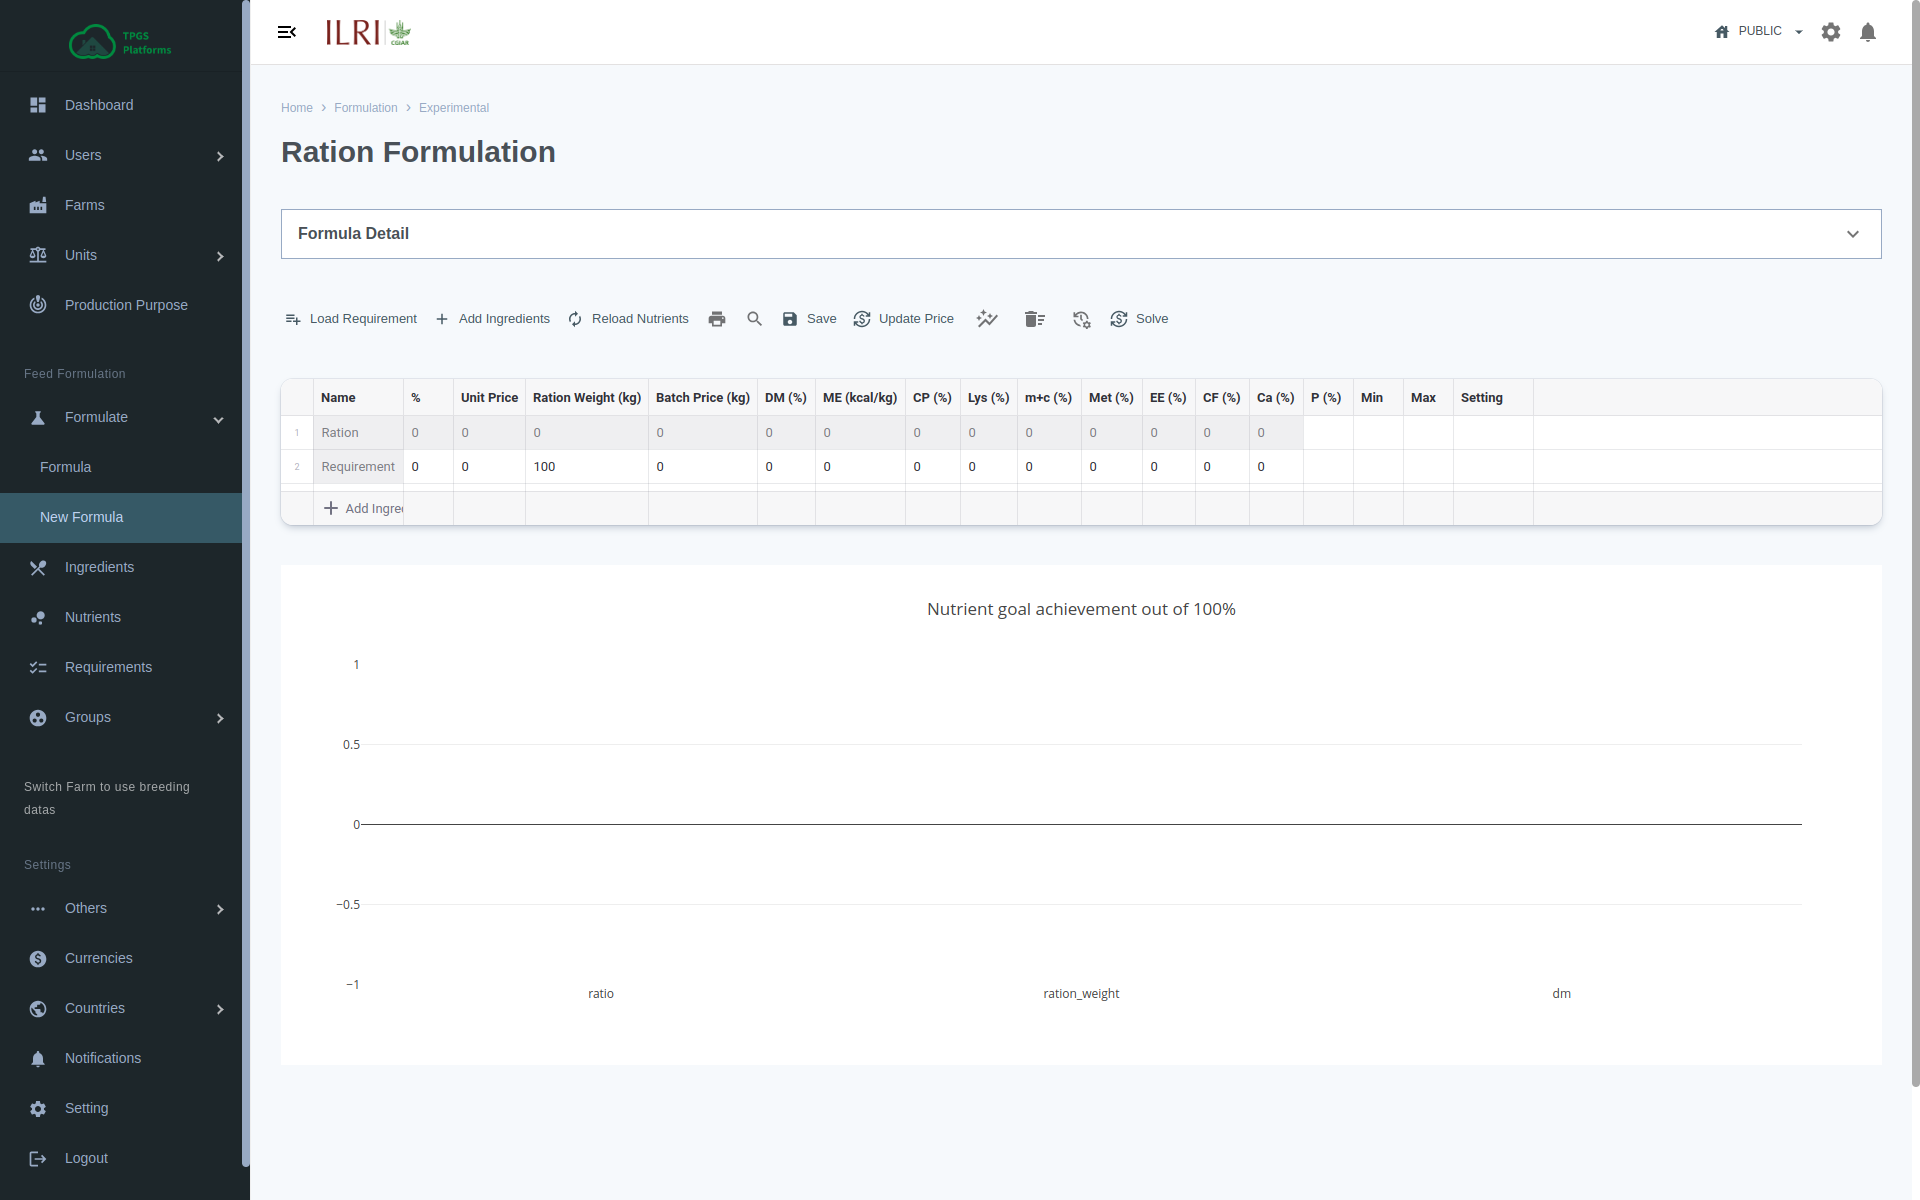
\includegraphics[width=15cm]{screenshots/ration_formulation_page.png}
  	\caption{Ration Formulation page}
  	\label{fig:ration_formulation_page}
\end{figure}

\paragraph{\arabic{stepcounter}.} Select the type of ration you want to prepare by clicking on \textcolor{ForestGreen}{"Load Requirement"}

\begin{figure}[h!]
  	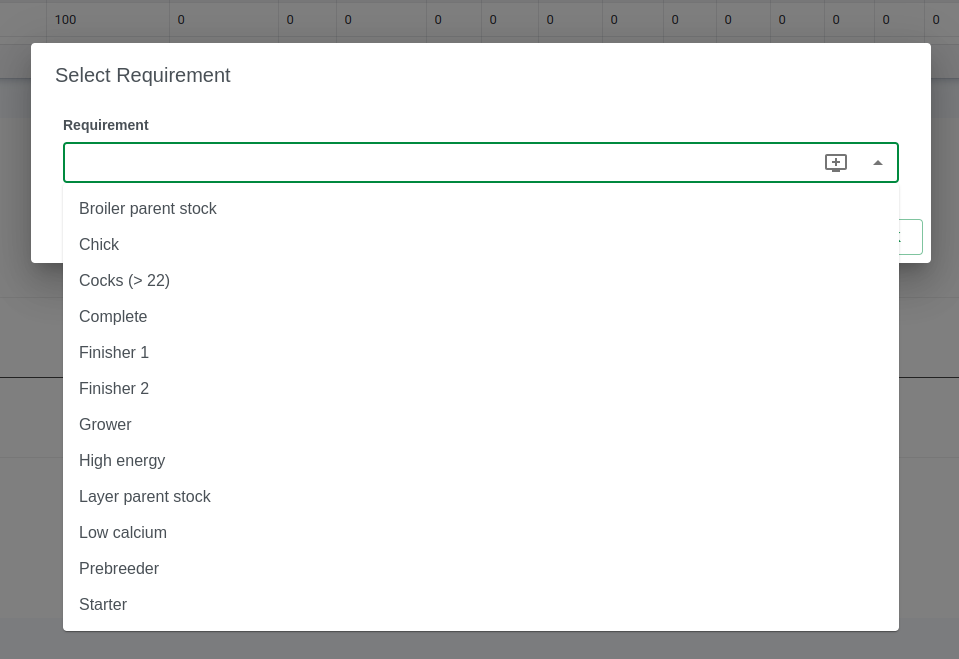
\includegraphics[width=15cm]{screenshots/load_requirement.png}
  	\caption{Load Requirement}
  	\label{fig:load_req}
\end{figure}

\paragraph{\arabic{stepcounter}.} Click \textcolor{ForestGreen}{"Add Ingredients"} to include the required ingredients.

\begin{figure}[h!]
  	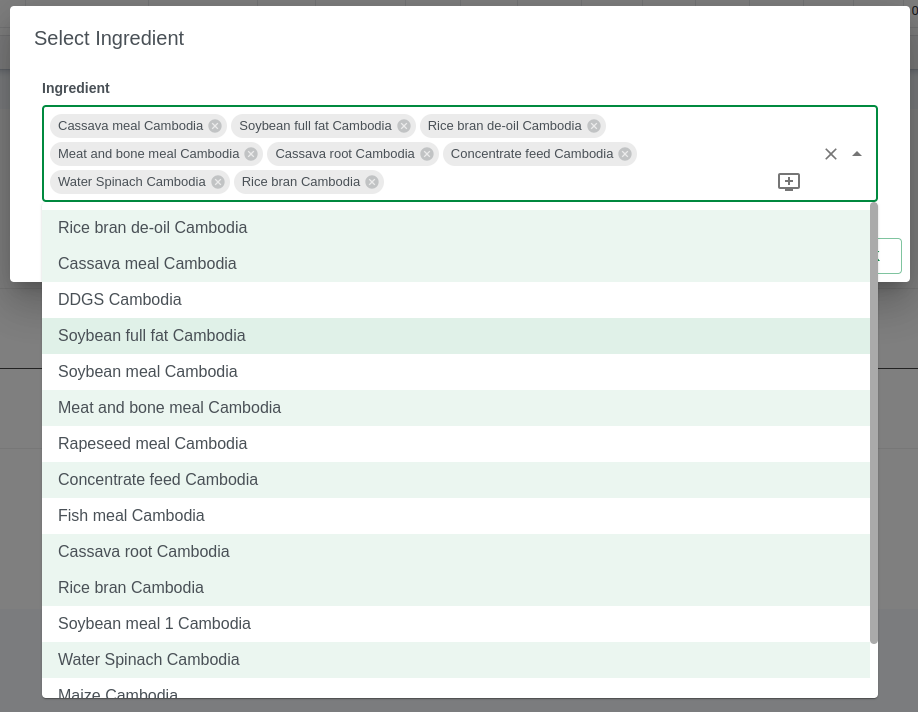
\includegraphics[width=15cm]{screenshots/select_ingredients.png}
  	\caption{Select multiple ingredients}
  	\label{fig:select_ing}
\end{figure}

\paragraph{\arabic{stepcounter}.} If the ingredient you want to include in you ration is not available Refere to \ref{sec:ingredient_create} 

\paragraph{\arabic{stepcounter}.}Formulate your ration ingredient type - \% per 100 kg, price (current price)

\paragraph{\arabic{stepcounter}.} Print or save (to keep it as an archive)

\paragraph{\arabic{stepcounter}.} To update the ingredients with the current price click “Update price”

Remark: If you want to do further analysis on formulated ration click the graph icon